\section{Durchführung}

Das verwendete Verfahren spiegelt ein Shadow Volumes artiges Verfahren im zweidimensionalen
Raum wieder. Auch hier wird die Silhouette des angestrahlten Rechtecks berechnet und and die
Grenzen, des Fensters auf dem Bildschirm, projiziert. Der von dieser Projektion abgedeckte
Bereich wird dunkler eingefärbt.

Der Rasterizer, welche die Schattenfläche auf die Lichtwerte der Pixel in dem Fenster anwendet,
benötigt zwei Strahlen, welche die Projektion der Silhouette darstellen, und ein Array von
Punkten welche alle Eckpunkte des Rechtecks, welche auf der dunklen Seite des Objektes liegen,
enthält. Diese werden benötigt, damit der Schatten das Rechteck nicht teilweise bis ganz
überdeckt. Somit kann man die Objekte in der Szene besser voneinander unterscheiden und sieht
nicht ausschließlich schwarze Flächen.

Es wird vor jeder Berechnung der Schatten von einem vollkommen beleuchteten Raum ausgegangen.
Dazu wird für jeden Pixel auf dem Bildschirm der Wert 1, von allen Lichtquellen beleuchtet,
gespeichert.

\begin{figure}[t]
	\centering
	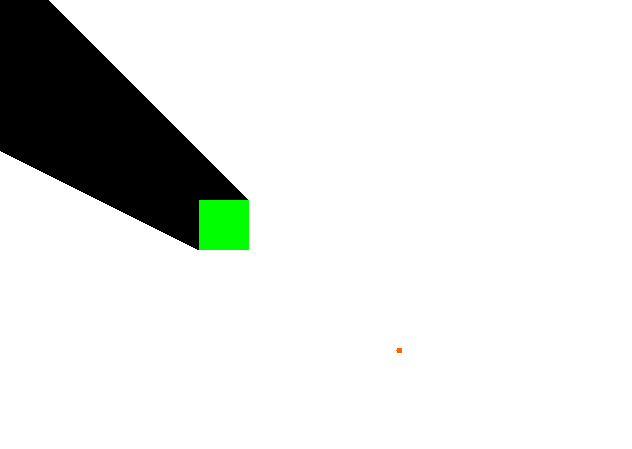
\includegraphics[width=\columnwidth]{images/durchfuehrung.png}
	\caption{einfacher Schatten}
	\label{fig:durch1}
\end{figure}

Im Folgenden wird die entwickelte Methode gezeigt um einen Schatten zu berechnen, wie er zum
Beispiel in Abbildung \ref{fig:durch1} zu sehen ist. Um diesen Schatten darstellen zu können
werden nun zuerst die zwei Strahlen durch Eckpunkte des schattenwerfenden Objektes berechnet,
die den größten Winkel zueinander haben.

\begin{figure}[t]
	\centering
	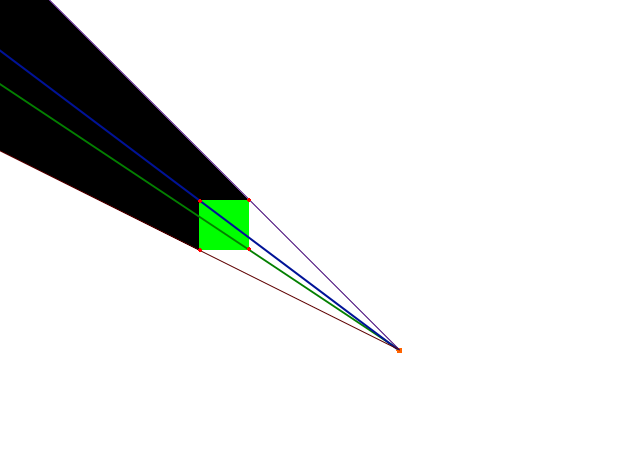
\includegraphics[width=\columnwidth]{images/durchfuehrung_1.png}
	\caption{Geraden durch Eckpunkte}
	\label{fig:durch2}
\end{figure}

Im ersten Schritt der Berechnung werden durch jeden Eckpunkt

\begin{equation}
	P = \left(\begin{array}{c} p_1 \\ p_2 \end{array}\right)
\end{equation}

des schattenwerfenden Objektes und die Position Lichtquelle

\begin{equation}
	L = \left(\begin{array}{c} l_1 \\ l_2 \end{array}\right)
\end{equation}

Geraden mit Ortsvektor, Position des Eckpunktes, und Richtungsvektor, Position der Lichtquelle,
subtrahiert von der Position des Eckpunktes

\begin{equation}
	\vec{g} = \left(\begin{array}{c} p_1 \\ p_2 \end{array}\right) + r \cdot \left(\begin{array}{c} p_1 - l_1 \\ p_2 - l_2 \end{array}\right)
\end{equation}

gelegt (Abbildung \ref{fig:durch2}).

\begin{figure}[t]
	\centering
	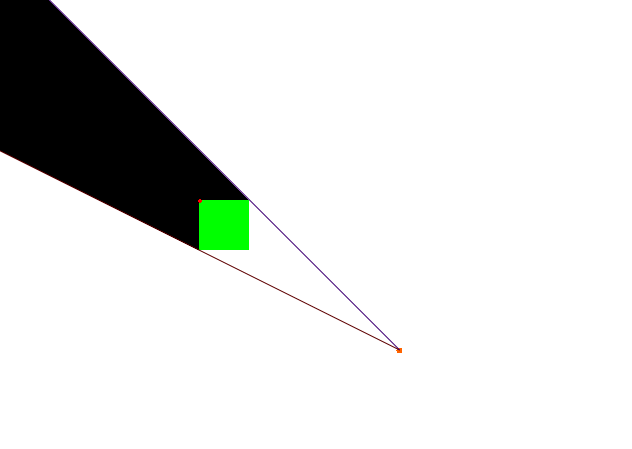
\includegraphics[width=\columnwidth]{images/durchfuehrung_4.png}
	\caption{Geraden mit größtem Winkel}
	\label{fig:durch3}
\end{figure}

%\vec{e}_1=\left(\begin{array}{c} 1 \\ 0 \end{array}\right)

Ausschlaggebend für die Silhouette des geworfenen Schatten sind die zwei Geraden, deren Winkel am
weitesten auseinander liegt (Abbildung \ref{fig:durch3}). Dazu wird rekursiv jedes Geradenpaar

\begin{equation}
	\vec{g}_1 = \vec{o}_1 + r \cdot \vec{m}_1, \vec{g}_2 = \vec{o}_2 + s \cdot \vec{m}_1
\end{equation}

durch den Winkel zwischen den beiden Richtungsvektoren der Geraden

\begin{equation}
	\omega = \arccos{\left(\frac{\vec{m}_1 \cdot \vec{m}_2}{|\vec{m}_1| \cdot |\vec{m}_2|} \right)}
\end{equation}

mit dem vorherig größten Geradenpaar verglichen und das mit dem größeren Winkel zurückgegeben.

\begin{figure}[t]
	\centering
	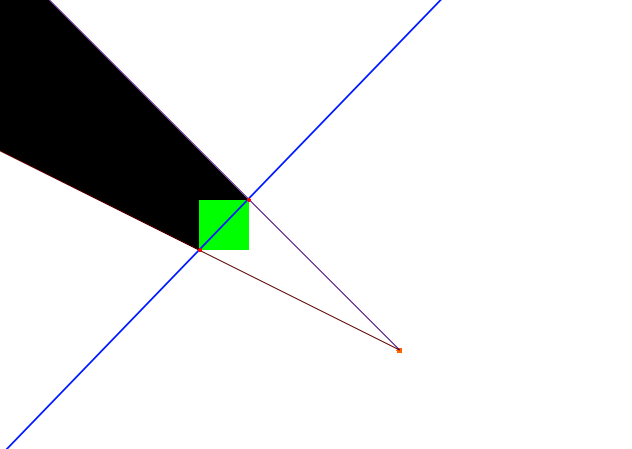
\includegraphics[width=\columnwidth]{images/durchfuehrung_2.png}
	\caption{Gerade durch Ortsvektoren}
	\label{fig:durch4}
\end{figure}

Damit später die Objekte nicht vom eigenen Schatten teilweise bis ganz überdeckt werden, werden nun
die Eckpunkte des Rechtecks berechnet, welche auf der dunklen Seite des Objektes liegen. Dazu wird
eine Gerade durch die Ortsvektoren der zwei vorher bestimmten Geraden bestimmt (Abbildung
\ref{fig:durch4}).

\begin{equation}
	s: \vec{s} = \vec{o}_1 + t \cdot \left(\begin{array}{c} o_{21} - o_{11} \\ o_{22} - o_{12} \end{array}\right)
\end{equation}

\begin{figure}[t]
	\centering
	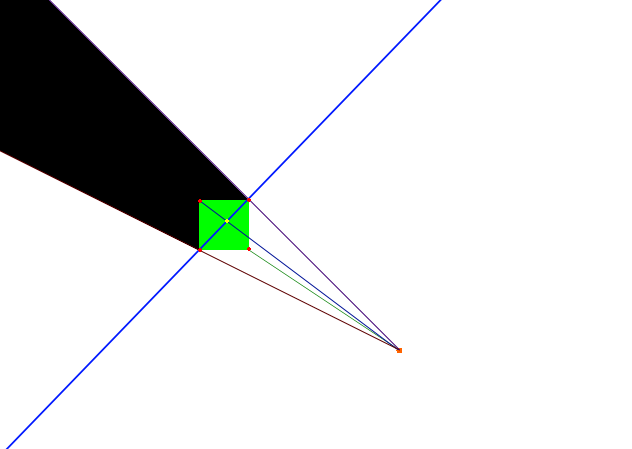
\includegraphics[width=\columnwidth]{images/durchfuehrung_3.png}
	\caption{Eckpunkte auf der dunklen Seite}
	\label{fig:durch5}
\end{figure}

Wenn ein Schnittpunkt zwischen der Geraden $s$ und der Strecke zwischen einem Eckpunkt des Rechtecks
und der Position der Lichtquelle vorhanden ist hängen wir diesen Eckpunkt an das an den Rasterizer
zu übergebende Array an (Abbildung \ref{fig:durch5}).

Durch die Arbeitsweise des Rasterizers müssen die Schnittpunkte der zwei Silhouettenstrahlen mit den
Fenstergrenzen nicht berechnet werden. Dieses Schattenmodell, bestehend aus zwei Strahlen und einem
Array an Punkten, kann an den Rasterizer übergeben werden.

Der Rasterizer wendet dieses Konstrukt mit Hilfe des aktive Kantenlisten Algorithmus auf die
Lichtwerte der Pixel in der Szene an. Der aktive Kantenlisten Algorithmus erlaubt eine inkrementelle
Berechnung der Schnittpunkte zwischen Polygonkanten und Pixelzeilen und somit wie weit ein Pixel
eingefärbt wird. Dazu wird eine Tabelle erzeugt, die für jede Pixelzeile eine Liste an aktiven Kanten
enthält. Diese aktiven Kanten enthält die x-Koordinate $x$ des Schnittpunktes mit der Bildzeile, die
Differenz zwischen den x-Koordinaten der Schnittpunkte $\Delta x$ zweier vertikal benachbarter
Geraden und die Anzahl der Bildzeilen $n_y$, die von der Polygonkante noch geschnitten werden. Nun
werden die Bildzeilen inkrementell durchlaufen. Dabei werden die Kanten in einer Bildzeile nach $x$
des Schnittpunktes aufsteigend geordnet. Dann wird von $x$ der ersten Kante bis $x$ der zweiten Kante
jedes Pixel eingefärbt. Diese beiden Kanten werden inkrementiert und die nächsten beiden Kanten werden
betrachtet, bis keine Kanten mehr in der Bildzeile übrig sind. Dann wird die nächste Bildzeile
betrachtet. Eine Kanten wird inkrementiert indem die Kante in die nächsthöhere Bildzeile verschoben
wird, $x$ auf $x + \Delta x$ gesetzt und $n_y$ dekrementiert wird.


Durch die Beschaffenheit dieses Algorithmus muss für den übergebenen Schatten in vielen Fällen nicht das komplette Polygon ausgerechnet werden.
